% IEEE journal format (IEEEtran, journal mode), e.g. for IEEE Access.
% Sections are generated from paper/ijf/ by build_ieee.py; edit those, not sections/.
\documentclass[journal]{IEEEtran}
\usepackage[T1]{fontenc}
\usepackage{cite,amsmath,amssymb,graphicx,booktabs,siunitx,url,xcolor}
\usepackage[hidelinks]{hyperref}
\sisetup{group-separator={,},group-minimum-digits=4}
\graphicspath{{../figures/}}
% IEEEtran has no \paragraph spacing tuned for run-in heads; keep them compact
\makeatletter\renewcommand\paragraph{\@startsection{paragraph}{4}{\z@}{1.2ex plus .4ex}{-1em}{\normalfont\normalsize\itshape}}\makeatother

\begin{document}
\title{Strong Baselines, Data Provenance and Post-Development Evaluation of Daily Mandi Price Forecasts at National Scale}

\author{C~Rishitha, Karthikeya~Y, Ashwin~Tyagi and Kaushal~S%
\thanks{The authors are with the Department of Artificial Intelligence and Data Science, Amrita Vishwa Vidyapeetham, Coimbatore, India.}%
\thanks{Corresponding author: [to be completed].}}

\markboth{Manuscript submitted for review}{Rishitha \MakeLowercase{\textit{et al.}}: Daily Mandi Price Forecast Evaluation}

\maketitle

\begin{abstract}
We report a bounded, clean-source retrospective study of Indian mandi price forecasts, using a fixed historical panel and a small LightGBM search budget. Two cleaning variants are rebuilt with pre- and post-execution source, input and executable hashes. Training, selection and interval calibration use disjoint periods; evaluation covers four horizons in already observed 2026 data. Pooled MAE is 4.4--5.9\% below contemporaneous persistence. However, MASE is approximately 1.00--1.11 against training-period naive error scales and omits 4.4--4.5\% of rows without usable scales. These different denominators preclude universal superiority claims. Longer circular and non-circular block sensitivities retain the observed advantage, but limited seasons and serial dependence leave inferential coverage unvalidated. Older national-scale and source-completeness results are historical supporting evidence, not reproduced principal findings. A frozen-model issuance recorder supports future collection; outcomes and human statistical review remain pending.
\end{abstract}

\begin{IEEEkeywords}
Agricultural prices, Forecast evaluation, Reproducibility, Cleaning sensitivity, Scaled errors, Dependent observations
\end{IEEEkeywords}


\section{Introduction}\label{sec:intro}

Indian agricultural wholesale markets (\emph{mandis}) report minimum, maximum and modal prices by commodity and variety through AGMARKNET and public data mirrors.
These reports provide price information for farmers comparing markets and sale timing, but their value as forecasting data depends on reporting continuity, source completeness and the evaluation protocol.
The empirical question is how much a learned forecast improves on simply retaining the latest reported price, and how cautiously that improvement should be interpreted.

The mandi forecasting literature includes studies of individual markets, small groups of markets and monthly indices (Section~\ref{sec:related}), often comparing deep or hybrid models with ARIMA \cite{paul2022brinjal,manogna2025deep,kumar2021onion}.
Forecast-evaluation research motivates a complementary emphasis: strong simple benchmarks \cite{makridakis2018statistical,makridakis2020m4}, appropriate scaling across heterogeneous series \cite{hyndman2006another}, alignment between the training loss and the scoring function \cite{gneiting2011making,kolassa2016evaluating}, and explicit treatment of leakage and data vintage \cite{hewamalage2022pitfalls,bokun2023fredsd}.
These considerations motivate an auditable empirical study rather than a claim of model superiority across published studies with different data and protocols.

Our primary contribution is a smaller, resource-limited \emph{clean-source release study} of daily mandi modal-price forecasting.
For each horizon and filtering regime, the learner uses \num{500000} deterministically sampled training rows from 2024; January--June 2025 is used for model selection and early stopping, July--December 2025 for interval calibration, and January--October 2026 for retrospective evaluation.
Targets are purged at period boundaries.
The release documents the feature builds and saved predictions, but retains a fixed historical panel as an external input.
It therefore supports claims about this release and observed panel, rather than validation of the earlier full national benchmark.

We make three empirical contributions, with their limits stated alongside the findings.
\begin{enumerate}
  \item \textbf{A chronological, baseline-explicit release comparison.}
    We compare an absolute-loss LightGBM candidate with persistence and four other simple baselines at the next-report, 3-, 7- and 14-day horizons.
    The two regimes exclude or retain reports flagged by the fivefold jump rule while preserving the other validity checks and panel membership.
    Across the eight fits, pooled MAE is 4.4--5.9\% lower than persistence on the retrospective evaluation rows.
    These are descriptive historical gains; adoption of LightGBM remains exploratory, with no independent confirmation of its superiority over the earlier Spark models or of benefits to farmer decisions.
  \item \textbf{Explicit separation of pooled error and scaled error.}
    Pooled MAE and MASE answer different questions: MASE divides errors by each series' training-period, horizon-specific naive error scale, whereas the pooled MAE comparison uses evaluation-period persistence error as its reference.
    MASE also omits approximately 4.4--4.5\% of forecast rows because their training scales are not positive and finite.
    It consequently describes a different population from full-row MAE; a MASE value above one is compatible with a pooled MAE gain over evaluation-period persistence.
  \item \textbf{Dependence-aware sensitivity analysis and interval assessment.}
    We report calendar-day block-resampling and dependence sensitivities alongside retrospective prediction-interval coverage.
    Forecast rows are not independent replicates, and the inference relies on approximate weak-dependence and stationarity assumptions conditional on the fitted models and observed panel.
    Neither small test probabilities nor narrow resampling intervals establish validated inferential coverage or generalisation to independent new markets.
\end{enumerate}

An earlier source-completeness audit provides historical supporting evidence that incomplete public mirrors can alter apparent forecast accuracy and interval coverage.
That audit is not reproduced as the principal validation of this release, and the release does not establish the original full benchmark's source state.
Similarly, the 2026 evaluation is retrospective: its forecasts were not issued as the reports arrived, so it does not constitute prospective confirmation.
Independent confirmation, expert statistical review and future-issued evaluation remain outstanding.

\section{Related work}\label{sec:related}

\paragraph{Forecasting across markets and horizons.}
Daily mandi forecasting studies establish the relevance of nonlinear learners but differ substantially in coverage and evaluation. Paul et al. compare ARIMA, GRNN, SVR, random forests and boosting for brinjal in 17 Odisha markets, including predictive-accuracy tests \cite{paul2022brinjal}. At broader coverage, monthly prices for 19 commodities in 143 markets favour recurrent models over alternatives including a random walk with drift \cite{paul2025deep}; daily data for 23 commodities in 165 markets are evaluated with an 80/20 split without MASE \cite{manogna2025deep}. Monthly aggregation, commodity selection and split design prevent direct numerical comparison with daily, target-purged multi-horizon evaluations. Hybrid, wavelet and neural models address individual commodity settings \cite{paul2021wavelet,jha2012tdnn,jha2013ann,anjoy2017pulses,kumar2021onion,praveenkumar2024potato,jaiswal2021lstm}, while combination methods also appear in agricultural forecasting \cite{wang2022bee}. Model complexity alone is therefore not a research contribution.

\paragraph{Evaluation and data provenance.}
Forecasting competitions motivate strong simple benchmarks \cite{makridakis2018statistical,makridakis2020m4,makridakis2022m5}. Scaled errors \cite{hyndman2006another}, predictive-accuracy tests \cite{diebold1995comparing} and time-series evaluation studies \cite{bergmeir2018note,cerqueira2020evaluating,hewamalage2022pitfalls} address complementary aspects of evaluation; a small p value cannot replace an effect size or evidence from an independent period. Consistency between training loss and the scored functional matters when many changes are zero \cite{gneiting2011making,kolassa2016evaluating}.
AGMARKNET missingness and erroneous entries have already motivated forecasting frameworks \cite{jain2020agmarknet,guo2020agmarknet}; we do not claim to discover agricultural data-quality problems. Real-time data vintages can also change macroeconomic forecast evaluations \cite{bokun2023fredsd}. Here the narrower question is whether incomplete mirror coverage changes agricultural evaluation on matched origins when compared with official reports.

\paragraph{Uncertainty and decision support.}
EnbPI, ensemble conformalised quantile regression and adaptive conformal inference address dependent observations \cite{xu2023conformal,jensen2024encqr,gibbs2021adaptive}. Drift-aware conformal prediction has already been applied to Chinese potato prices \cite{ouyang2026potato}; our volatility-stratified split-conformal implementation is an evaluated baseline, not a new uncertainty method. Selection and calibration sharing a period in the original experiment motivates the separate-period robustness study below. Information interventions have heterogeneous effects on farmers \cite{jensen2007digital,goyal2010information,fafchamps2012sms,mitra2018asymmetric}, so price-prediction gains cannot establish welfare or trading profits.

\paragraph{Contribution and scope.}
The primary contribution is a bounded, clean-source cleaning and dependence-sensitivity study on a fixed historical panel. It documents a small-budget comparison with five simple baselines, disjoint selection/calibration periods, multiple metric denominators and explicit dependence limitations. This is an empirical execution/evaluation contribution, not a new learner, novel conformal method or claim of unprecedented combination. The earlier matched-origin source-completeness audit is historical supporting motivation, not the principal reproduced validation. Model adoption remains exploratory, and retrospective gains are not independently confirmed.

\paragraph{Implication for research practice.}
A small-budget study should distinguish pooled rupee gains from scaled errors, preserve unfavorable groups, disclose dependence assumptions and separate source-attributable execution from independent future confirmation. Historical source audits additionally motivate checking coverage before attributing error changes to market drift. These are practical evaluation lessons, not causal findings or new statistical theory. The value of this narrower contribution must be judged against the target venue's expectations, rather than inferred from dataset scale or a model label.

\section{Retained data and fixed-panel scope}\label{sec:data}
The primary experiment uses retained silver v2 mandi reports, combining the AGMARKNET Kaggle archive before October 2025 with official data.gov.in reports thereafter. Prices are INR per quintal. Input Parquet bytes and shard lists are hashed before and after feature execution; these retained bytes, rather than an assurance of identical later API responses, define the reproduced dataset. Official resource access requires a key, which is excluded from source and archives.

The 36-commodity panel is an existing table of 11,845 eligible market--commodity--variety series, supplied as a fixed, hashed external input. Its original selection is not reproduced or independently certified here. Depending on horizon and cleaning regime, the evaluation contains 4,602--5,182 series, rather than all panel members. Findings apply to these eligible report-days and cannot represent every Indian market or farmer.
Both cleaning variants are newly built from the same inputs, with history beginning 2022-10-01, for warm-up before 2024 training. The cleaned variant removes reports flagged by a fivefold deviation from the prior ten-report geometric mean; the unfiltered variant retains them. Other validity checks, harmonisation, panel and build settings are held fixed. This does not create manual error labels: unusual prices can be genuine. Common origins may still carry different targets and features after filtering, so the comparison is pipeline sensitivity, not a causal effect of cleaning.

Build records bind the committed source, executed assembly JAR, commands, runtime versions and exit codes to output checksums. This is observed execution attestation, not an independent build witness. Large inputs are retained locally outside Git; a public immutable archival package and independent-environment reproduction remain outstanding. The earlier national-scale source audit and full-size experiments are historical supporting material in the historical supplement, not acceptance-critical validation of this primary study.

\section{Forecasting task and evaluation protocol}\label{sec:protocol}

\paragraph{Task.}
Entity $e$ reports modal prices $P_{e,t}$ (INR per quintal) on irregular dates.
For an origin $t$ and $h\in\{3,7,14\}$ days, the target is the first report dated in $[t+h,t+h+3]$. If there is none, there is no label.
The \emph{next} horizon is the next report, if it falls within 7 days.
Models predict $y=\ln P_{e,\tau}-\ln P_{e,t}$, and errors are measured in rupees on $P_{e,t}\exp(\hat y)$.

\paragraph{Periods (main experiment).}
\begin{itemize}
  \item Training origins: 2016--2023.
  \item Validation: 2024, used for tuning, model choice and conformal calibration.
  \item Test origins: 2025-01-01 to 2026-04-20, scored once.
\end{itemize}
A row is kept only if its target date also lies in its period; a unit test enforces this purge.
A perturbation test multiplies all future prices, and all other entities' prices, by arbitrary factors and requires every feature at the origin to be unchanged.
Training uses a uniform sample of $2\times10^6$ rows per horizon (fixed seed).

\paragraph{Selection.}
The family with the lowest validation MAE is selected, baselines included.
The search space was amended twice, both times on validation evidence, before any test metric was read:
\begin{itemize}
  \item first, after squared-loss learners tied persistence;
  \item second, after finding that MLlib's absolute-loss boosting is mis-scaled for log returns.
\end{itemize}
An aborted first run had already written test predictions for one horizon. They were deleted unread, and we disclose this.

\paragraph{Metrics and tests.}
We report:
\begin{itemize}
  \item MAE, RMSE, WAPE, sMAPE and bias;
  \item MASE, scaled by each entity's in-sample $h$-step naive MAE on training rows \cite{hyndman2006another};
  \item MAE relative to persistence on identical rows;
  \item the share of series (at least 30 test rows) on which a model beats persistence.
\end{itemize}
Diebold--Mariano tests \cite{diebold1995comparing} use daily mean absolute-error differences, a Newey--West variance with lag $h+3$ (7 for the next report) and the HLN correction. Same-day errors are aggregated first because they are correlated across markets.

\paragraph{Frozen-model and retraining evaluations.}
After the official back-fill, we score the frozen models, quantiles and MASE scales on complete official data:
\begin{itemize}
  \item on the original test period;
  \item on 2026-04-22 to 2026-10-22, reports first downloaded after the models were saved.
\end{itemize}
Separately, we retrain with the same search space, selection rule, sample size and seed, on a protocol fixed before the run:
\begin{itemize}
  \item training: 2016--2024;
  \item validation: 2025;
  \item final test: 2026-01-01 to 2026-10-22, not used for any retraining choice. Its first months overlap the main test, and its later months had already been used to score the frozen models.
\end{itemize}

\section{Methods}\label{sec:methods}

\paragraph{Features.}
Each origin carries 24 base features plus one horizon-specific seasonal feature, all computed from reports dated $\le t$ (Table~\ref{tab:features}).
Missing numeric values are set to zero; reporting counts and seasonal availability indicators provide partial missingness context. The commodity vocabulary is fitted on training rows.
The cross-market features use other markets' reports of the \emph{same day}, which assumes those are published by the end of day $t$.
The older historical study examined previous-day cross-market features; that ablation is not rerun in this bounded experiment.

\begin{table*}[!t]\centering\small
\caption{Feature groups ($\ell=\ln P$); all frames end at the origin.}\label{tab:features}
\begin{tabular}{@{}lp{0.72\linewidth}@{}}\toprule
Group & Features\\\midrule
Level and lags & $\ell_t$; differences to the 1st, 2nd and 5th previous reports; days since the previous report\\
Rolling (7/30/90 d) & deviation from the rolling mean; standard deviation (30, 90); report counts (30, 90); distance to the 30-day max and min\\
Range & $(\max-\min)/\text{modal}$ on day $t$\\
Seasonal & deviation from the level at $t-365\pm3$; availability indicator; last year's change from $t-365$ to $t+h-365$\\
Cross-market & same-day mean 30-day deviation and last return of the commodity, nationally and within the state; number of reporting markets\\
Calendar & day of year (sine, cosine); day of week\\
Categorical & commodity\\\bottomrule
\end{tabular}\end{table*}

\paragraph{Baselines and learner.}
The five baselines are persistence, 7/30-day geometric rolling averages, seasonal naive with persistence fallback, and seasonal-adjusted persistence using last year's horizon change. They are evaluated on the same eligible rows as the candidate. SES, MLlib and three-seed LightGBM comparisons belong to the older historical study and are not rerun or claimed independently confirmed here.
Each horizon/variant trains a LightGBM L1 log-return model with learning rate 0.05, minimum leaf size 200, feature fraction 0.8 and bagging fraction 0.7. Early stopping uses selection-period log-return L1 loss; leaf count is selected by rupee MAE on that period. One seed and a deliberately small search budget bound this study; they do not establish best possible predictive performance or training stability.

\paragraph{Price intervals.}
Only calibration-period residuals and 30-day log-price volatility define the five volatility bins and residual quantiles. The 5/10/90/95\% quantiles produce nominal 80/90\% price intervals. This implements a baseline residual calibration, not new conformal methodology. Temporal dependence and changing distributions prevent an exchangeability-based coverage guarantee \cite{gibbs2021adaptive}; coverage is measured retrospectively, not promised for future prices.

\section{Primary clean-source study results}\label{sec:point}
\paragraph{Clean-source release-study results.}
This is a new end-to-end execution of the smaller study, with identical historical periods and model search budget; it is not an exact replication of the full-size historical experiment. The pre-build source tag is \texttt{agdata-research-source-v1}. Both feature tables were rebuilt, with source/input/executable snapshots checked before and after execution. The fixed historical panel is an explicitly hashed external input, not a reproduced panel-selection process. Source attribution is stronger than in the earlier runs, but an observed execution log is not an independent build witness. All results remain retrospective and conditional on the fitted models and observed panel.
Across the eight fits, observed pooled MAE reductions are 4.4--5.9\%, or INR 9.92--18.83 per quintal. Table~\ref{tab:release_point} gives absolute errors and exposure. These gains are descriptive historical differences, not evidence of profitable farmer decisions or independent LightGBM superiority over Spark models. MASE excludes 4.4--4.5\% of rows lacking positive finite training scales, and therefore describes a different population from full-row MAE.

\begin{table*}[!t]\centering\small\setlength{\tabcolsep}{3pt}
\caption{Clean-source release study: candidate/persistence MAE in INR per quintal, forecast rows, calendar days and MASE-excluded rows. Forecast rows are not independent replicates.}\label{tab:release_point}
\begin{tabular}{@{}llrrrrr@{}}\toprule
Regime & Horizon & Rows & Days & MAE C/P & Rel. MAE & MASE omitted\\\midrule
cleaned & next & 553,793 & 294 & 192.34/202.26 & 0.951 & 24,276 \\
cleaned & h3 & 531,316 & 292 & 238.61/252.95 & 0.943 & 24,008 \\
cleaned & h7 & 519,244 & 288 & 301.36/317.31 & 0.950 & 22,739 \\
cleaned & h14 & 496,298 & 281 & 393.48/411.51 & 0.956 & 22,305 \\
unfiltered & next & 554,112 & 294 & 197.04/207.30 & 0.951 & 24,292 \\
unfiltered & h3 & 531,606 & 292 & 243.52/258.90 & 0.941 & 24,024 \\
unfiltered & h7 & 519,527 & 288 & 307.13/323.36 & 0.950 & 22,756 \\
unfiltered & h14 & 496,581 & 281 & 397.39/416.21 & 0.955 & 22,321 \\
\bottomrule\end{tabular}

\end{table*}

\begin{table*}[!t]\centering\small\setlength{\tabcolsep}{3pt}
\caption{Circular-block relative-MAE percentile sensitivity intervals (2,000 replicates, nominal 95\%). Actual coverage is unvalidated; all block specifications are shown.}\label{tab:release_circular}
\begin{tabular}{@{}llrrr@{}}\toprule
Regime & Horizon & 28 days & 42 days & 56 days\\\midrule
cleaned & next & [0.947, 0.955] & [0.947, 0.955] & [0.947, 0.955] \\
cleaned & h3 & [0.940, 0.948] & [0.940, 0.947] & [0.940, 0.947] \\
cleaned & h7 & [0.946, 0.953] & [0.946, 0.953] & [0.946, 0.953] \\
cleaned & h14 & [0.952, 0.961] & [0.953, 0.961] & [0.953, 0.960] \\
unfiltered & next & [0.945, 0.955] & [0.946, 0.955] & [0.946, 0.955] \\
unfiltered & h3 & [0.936, 0.946] & [0.936, 0.945] & [0.936, 0.945] \\
unfiltered & h7 & [0.946, 0.954] & [0.946, 0.954] & [0.946, 0.954] \\
unfiltered & h14 & [0.949, 0.960] & [0.950, 0.959] & [0.952, 0.958] \\
\bottomrule\end{tabular}

\end{table*}

\begin{table*}[!t]\centering\small\setlength{\tabcolsep}{3pt}
\caption{Non-circular-block sensitivity intervals under the same settings. Long blocks leave few temporal spans and do not establish stationarity or future transportability.}\label{tab:release_noncircular}
\begin{tabular}{@{}llrrr@{}}\toprule
Regime & Horizon & 28 days & 42 days & 56 days\\\midrule
cleaned & next & [0.946, 0.955] & [0.946, 0.955] & [0.947, 0.955] \\
cleaned & h3 & [0.939, 0.947] & [0.939, 0.947] & [0.940, 0.947] \\
cleaned & h7 & [0.946, 0.954] & [0.946, 0.953] & [0.946, 0.952] \\
cleaned & h14 & [0.952, 0.962] & [0.952, 0.961] & [0.953, 0.959] \\
unfiltered & next & [0.946, 0.956] & [0.946, 0.955] & [0.947, 0.955] \\
unfiltered & h3 & [0.938, 0.946] & [0.939, 0.946] & [0.939, 0.946] \\
unfiltered & h7 & [0.946, 0.955] & [0.947, 0.955] & [0.947, 0.954] \\
unfiltered & h14 & [0.951, 0.961] & [0.952, 0.960] & [0.953, 0.958] \\
\bottomrule\end{tabular}

\end{table*}
The sensitivity interval endpoints across all six specifications and eight fits span 0.936--0.962; this range is not a combined confidence interval. State and commodity summaries contain 46 group-by-fit comparisons with relative MAE above one; all subgroup counts and errors are retained, without selecting favourable subgroups. Groups and fits overlap, so this count is descriptive, not a multiplicity-adjusted finding.

The daily diagnostics in Figure~\ref{fig:release_dependence} display loss differences, exposure and autocorrelation for the cleaned 7-day fit; diagnostics for all fits are recorded with the release. Substantial long-range correlation, seasonal changes or exposure variation can invalidate short-memory approximations. HAC bandwidth sensitivity is secondary: no horizon correction is claimed and tiny p values are not evidence of validated inference. Independent entity-resampling intervals are exploratory and cannot establish generalisation to independent new markets. Human expert statistical review and genuinely future-issued evaluation remain outstanding.
\begin{figure}[!t]\centering
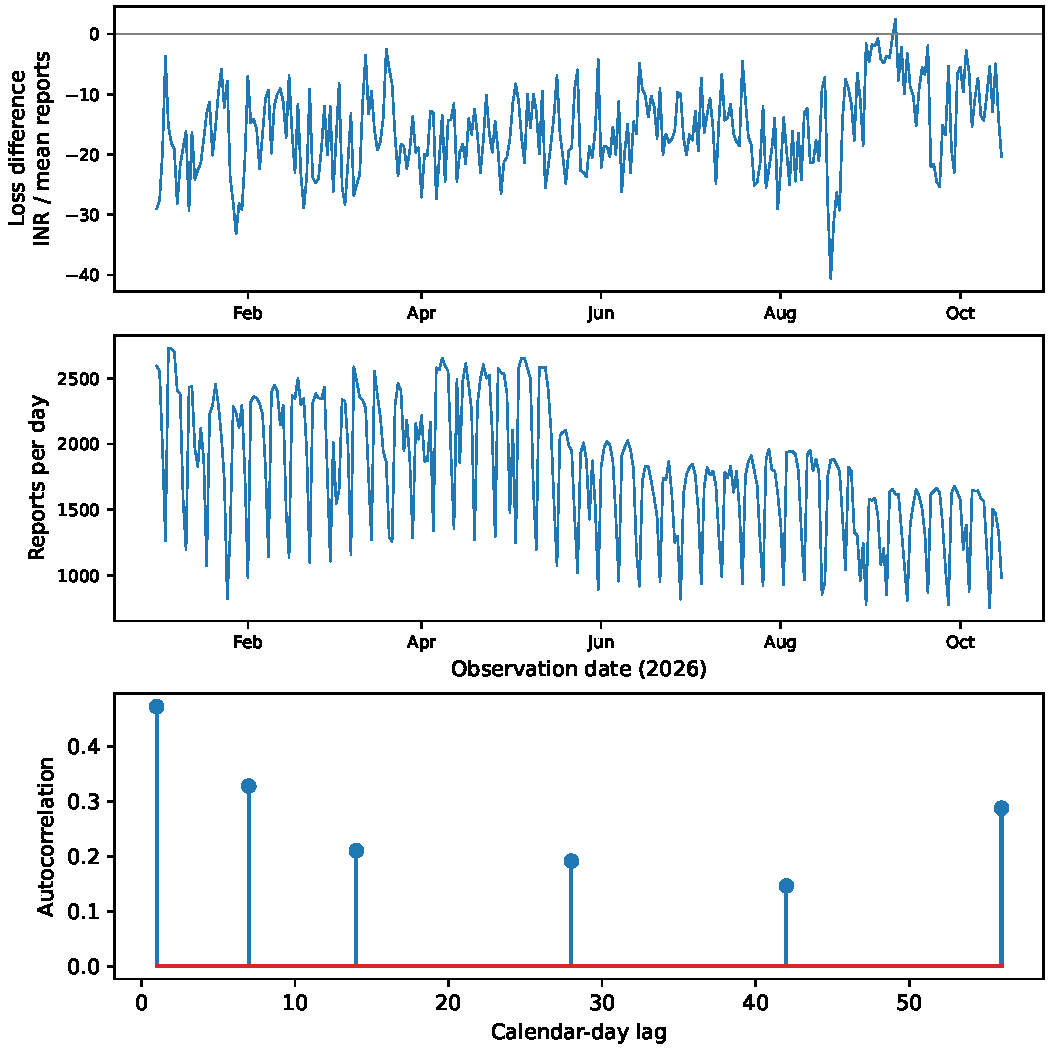
\includegraphics[width=0.88\linewidth]{release_dependence.pdf}
\caption{Release cleaned 7-day daily candidate-minus-persistence total loss divided by mean daily exposure (top), report counts (middle), and descriptive autocorrelation (bottom). No independence threshold is asserted.}\label{fig:release_dependence}
\end{figure}


\section{Interval calibration and the data-provenance effect}\label{sec:intervals}

\paragraph{Main test.}
On the main test, empirical coverage of the nominal 80\% intervals is 78.6\%, 79.4\%, 80.0\% and 80.5\% for the four horizons; for the 90\% intervals it is 88.9--90.5\%.
Across volatility quintiles, coverage stays within 77.2--82.0\%.
Interval widths adapt strongly, from 2--8\% of the price in the calmest quintile to 45--88\% in the most volatile (Figure~\ref{fig:cov}).

\begin{figure}[!t]\centering
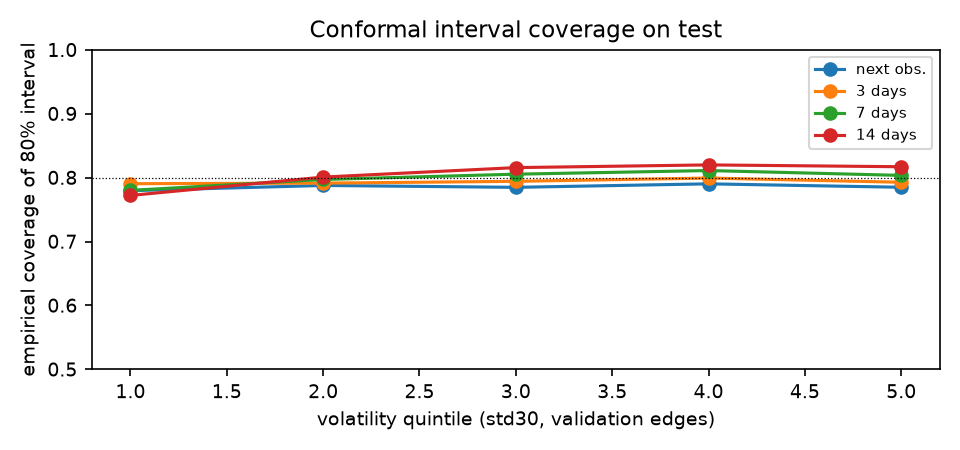
\includegraphics[width=\columnwidth]{interval_coverage.png}
\caption{Test coverage of 80\% split-conformal intervals by volatility quintile (bin edges from validation).}\label{fig:cov}
\end{figure}

\paragraph{Provenance effect.}
Measured on the mirror after the November 2025 portal change:
\begin{itemize}
  \item 80\% coverage fell to 67.6--72.9\%;
  \item relative MAE weakened to 0.993, 0.977, 0.968 and 0.944.
\end{itemize}
This had the hallmarks of a distribution shift.
Re-scoring the \emph{same frozen models} on the complete official record for the same period (Table~\ref{tab:prov}) gives:
\begin{itemize}
  \item coverage of 78.0--78.7\%, a loss of only 1.2--2.2 points against the pre-change period;
  \item relative MAE of 0.976, 0.962, 0.962 and 0.937.
\end{itemize}
The two record sets differ in which rows exist: after the change the mirror has only 62,845--97,079 test rows per horizon, against 332,275--391,425 officially.
We therefore also score both on the identical (series, origin) keys present in both (50,923--78,773 rows per horizon; last block of Table~\ref{tab:prov}).
On these identical rows, mirror coverage is 68.0--72.3\% and official coverage 78.8--79.7\%. The calibration loss is therefore not an artefact of sample composition.
Most of the apparent loss of calibration was produced by the mirror's missing reports.
Accuracy is a different matter. On official data the 7-day relative MAE still rises from 0.938 before the change to 0.962 after, so the gain over persistence shrinks from 6.2\% to 3.8\%. Part of the accuracy shift is real.
The mechanism is consistent with Section~\ref{sec:data}: three-times-longer gaps make ``next'' targets more distant and trailing windows sparser, so realised changes exceed what validation residuals calibrated on denser series anticipate.
A provenance audit is therefore a precondition for any claim about drift in this data.

\begin{table}[!t]\centering\small
\caption{Frozen models after the November 2025 portal change (2025-11-01 to 2026-04-20): mirror versus complete official record.}\label{tab:prov}
\begin{tabular}{@{}lrrrr@{}}\toprule
 & next & 3 d & 7 d & 14 d\\\midrule
Rel.\ MAE, mirror & 0.993 & 0.977 & 0.968 & 0.944\\
Rel.\ MAE, official & 0.976 & 0.962 & 0.962 & 0.937\\
80\% coverage, mirror & 67.6\% & 71.3\% & 72.0\% & 72.9\%\\
80\% coverage, official & 78.0\% & 78.7\% & 78.7\% & 78.5\%\\\midrule
\multicolumn{5}{@{}l}{\emph{Identical (series, origin) keys}}\\
Rel.\ MAE, mirror & 0.998 & 0.983 & 0.971 & 0.942\\
Rel.\ MAE, official & 0.972 & 0.958 & 0.959 & 0.930\\
80\% coverage, mirror & 68.0\% & 71.6\% & 71.9\% & 72.3\%\\
80\% coverage, official & 78.8\% & 79.7\% & 79.7\% & 79.3\%\\\bottomrule
\end{tabular}\end{table}

\section{Historical context and future-issued evaluation}\label{sec:prospective}
\paragraph{Supporting historical context.}
The separate historical supplement preserves earlier national-scale MLlib benchmarks, source-completeness comparisons, timing ablations, refits and decision-rule backtests. Their original full-size execution and panel selection have not been reproduced end-to-end. They are supporting history, not the primary contribution or validation of this bounded study. The historical matched-origin mirror/official comparison motivates source audits before interpreting drift; it does not isolate causal contributions of changed features, target reports or missingness.

\paragraph{Exploratory adoption boundary.}
The prototype's LightGBM serving choice used a period already examined during development. Neither this smaller experiment nor its cleaning variants independently confirms LightGBM superiority over newly refitted Spark alternatives. The primary question here is its observed performance against the five specified simple baselines under a recorded, bounded execution.

\paragraph{Future collection, not completed confirmation.}
A new local issuance utility copies and hashes the existing prototype boosters, feature/category metadata and calibration, records source and dependencies, and recomputes forecasts using those frozen artifacts. Only recent prior-day origins whose entire target window starts strictly after the local issuance date qualify. The CLI accepts no backdating override; feature-file hashes, future-date rejection, duplicate keys and a chained batch manifest support integrity checks. This future-window population can exclude next-report forecasts and differs from the retrospective-origin population, which must be reported rather than silently equated.
The frozen prototype is not the smaller release-study model, so this collection cannot directly confirm that model's future gain. The local system clock and hash chain are not external time attestation or proof of point-in-time raw-report availability. No outcomes are scored or future success assumed. At least 90 completed calendar days plus target maturation, a reviewed scoring protocol, independent archival and human statistical review remain required before any confirmatory interpretation. No issuance schedule is installed. The operational protocol and actual collection status are kept outside retrospective result tables.

\section{Discussion, limitations and practical meaning}\label{sec:discussion}
The primary evidence is a modest reduction of pooled rupee error under two cleaning pipelines in one already observed evaluation period. MASE near or above one, omitted scales and worse-performing subgroups constrain its interpretation. Some error gains may matter operationally, but modal price is a published market summary, not a farmer's transaction price; transport, fees, perishability and storage can outweigh these differences. No profit or welfare effect is estimated \cite{fafchamps2012sms,mitra2018asymmetric}.

The statistical sample includes 281--294 calendar days, not hundreds of thousands of independent trials. Shared shocks, overlapping targets, changing report counts and long-range autocorrelation complicate inference. A 56-day block yields only about five non-overlapping temporal spans; 2,000 resamples cannot create independent seasons. The sensitivity grid is useful disclosure, not validated coverage or a substitute for human statistical review. Independent entity resampling does not make correlated markets independent. Training-sample and hyperparameter-search uncertainty are not captured.

Other limitations are the fixed historical panel, one training year, one seed, two leaf settings, source revisions, irregular target availability, omitted weather/arrivals, and assumed end-of-day availability of same-day cross-market features. The evaluation year was visible during design. The clean execution is not independent confirmation or a reconstruction of the older national-scale benchmark. We do not extend the primary evaluation into the selection/calibration periods merely to obtain more observations: doing so would change their roles and would not add independent seasons. Longer independent observation requires time-forward collection or a separately defined rolling-origin study.

The main reproducibility claim is scoped to this smaller retained-input execution. A public immutable archive of exact large input bytes, a separate-environment run, and a human statistician's assessment remain outstanding. IJF is the intended empirical forecast-evaluation venue, not a claim of readiness or acceptance. We do not propose a new learner, new conformal theory, causal missingness effect or superiority over papers with incompatible data and protocols. The six-language prototype and historical decision cards are supporting system work, not experimentally demonstrated farmer benefit; native-speaker, device and farmer reviews remain pending.

\section{Conclusions and reproducibility boundary}\label{sec:conclusion}
A bounded, clean-source retrospective study shows 4.4--5.9\% lower pooled MAE than contemporaneous persistence across four horizons and two cleaning regimes. MASE remains approximately 1.00--1.11 using training-period scales, with 4.4--4.5\% of rows omitted only from that metric. The conclusion is modest historical average error reduction under specified settings, not universal predictive superiority or improved farmer profit.

The contribution is a reproducible small-budget cleaning/dependence sensitivity study on retained inputs. Historical national-scale comparisons and the source-completeness audit are separated as supporting material; their original full-size execution and panel selection are not certified by this work. Dependence sensitivities remain approximate and retrospective. Frozen-model future issuance can begin collecting a different, explicitly defined population, but no future confirmation or human statistical approval is claimed.

\paragraph{Artifacts and availability.}
Fitting source is tagged \texttt{agdata-}\allowbreak\texttt{research-}\allowbreak\texttt{source-v1}; release records bind pre/post source/input/JAR hashes, commands and feature outputs. Saved predictions and generated primary tables are recorded under \path{results/release_v1}. Models, large data and issuance batches remain local outside Git. Public source/results tags and compact manifests do not constitute a public immutable data archive, independently witnessed execution or anonymised journal submission package. Later API responses can differ from retained bytes after revisions. The fixed panel is a declared external input. Corresponding-author details, declarations and formal journal-template compliance remain unverified.

The evidence ledger, commands, third-review response and future protocol distinguish reproduced retrospective results, historical supporting evidence and pending forward evaluation. Human expert statistical review, independent archival/reproduction and completed prospective outcomes remain necessary before a stronger submission recommendation.


\section*{Acknowledgment}
The authors thank Dr.~Sreeja (Amrita Vishwa Vidyapeetham) for guidance. AGMARKNET data are published by the Government of India under the GODL-India licence.

\bibliographystyle{IEEEtran}
\bibliography{../references}
\end{document}
